\section*{Introducción}
\noindent 
¿Cuál es la primera diferencia que encontramos entre la computación clásica y la cuántica? \\
\noindent 
La respuesta es sencilla y la diferencia está en la unidad de medida. \\[0.5em]
\noindent 
Cualquier función, procedimiento o cálculo que realice una computadora requiere el manejo de variables o parámetros, valores numéricos que se usan para realizar los cálculos correspondientes. En la computación clásica, la unidad básica de medida utilizada son los bits. Un bit sólo puede tomar dos valores posibles: 1 y 0.\\[0.5em]
\noindent 
Para entenderlo mejor, podríamos verlo como un interruptor donde el 0 representa "apagado" y el 1 representa "prendido". Sería ilógico pensar que un bit puede estar prendido y apagado a la vez. Otra manera de visualizarlo es con una moneda: cada moneda tiene lo que conocemos como “Cara” y “Escudo”. Si tiramos una moneda, caerá cara o escudo con un 50\% de probabilidad para cada resultado. Es importante tener este ejemplo en mente para explicar de mejor manera una característica fundamental de la computación cuántica.\\[0.5em]
\noindent 
Por otro lado, en la computación cuántica, la unidad de medida es el bit cuántico, abreviado como “qubit”. A diferencia del bit clásico, el qubit tiene una identidad más fluida y no binaria. Esto significa que un qubit no está limitado a tomar un único valor de 0 o 1. Por el contrario, gracias a la propiedad cuántica de la superposición, un qubit puede representar una combinación de 0 y 1 al mismo tiempo, con probabilidades específicas asociadas a cada uno. Esta idea puede generar confusión al principio, así que expliquemos con un ejemplo mas natural.
\noindent 
\subsection*{La Moneda Clásica vs. La Moneda Cuántica}

\subsection*{Moneda Clásica}
\noindent
En la computación clásica, si tiramos una moneda, caerá en alguna de sus dos caras: cara (1) o escudo (0). Es decir, la moneda solo puede estar en un estado claramente definido en cada momento. Cada vez que lancemos la moneda, obtendremos un resultado único y determinista. Si hacemos este experimento varias veces, por ejemplo, 100 veces, esperaremos ver aproximadamente 50 caras y 50 escudos, dado que la probabilidad de cada lado es del 50\%.

\subsection*{Moneda Cuántica}
\noindent
En la computación cuántica, una moneda "cuántica" no se comporta de la misma manera. Antes de medirla, no está estrictamente en cara ni en escudo. En cambio, está en un estado de \textbf{superposición} de ambos. Esto significa que la moneda cuántica puede representar simultáneamente un espectro de posibilidades de cara y escudo. Por ejemplo, podríamos describir este estado como:\\[0.5em]

\[
|\psi\rangle = \sqrt{0.8}|0\rangle + \sqrt{0.2}|1\rangle
\] \\[0.5em]

\noindent
Aquí, \( |\psi\rangle \) es el estado cuántico de la moneda, y los coeficientes \( \sqrt{0.8} \) y \( \sqrt{0.2} \) representan las amplitudes de probabilidad para los estados \( |0\rangle \) (escudo) y \( |1\rangle \) (cara), respectivamente. Al medir la moneda, hay un 80\% de probabilidad de obtener escudo y un 20\% de probabilidad de obtener cara.
Hasta que no la medimos, está en este estado de superposición, no se preocupen si ven muy raros estos símbolos, en los siguientes capítulos se explicará de una manera clara.\\[0.5em]
\noindent
Imaginemos también que visualizamos la moneda no como un objeto estático, sino como una esfera (la esfera de Bloch) donde cada punto en la superficie representa un posible estado cuántico, con combinaciones específicas de 0 y 1, como se puede visualizar en la figura~\ref{fig:esferaBloch}. En la computación clásica, el estado de un bit es determinista: siempre es 0 o 1, nunca ambos. En cambio, en la computación cuántica, un qubit puede estar en ambos estados simultáneamente hasta que lo medimos.\\[0.5em]
\begin{figure}[h!]
    \centering
    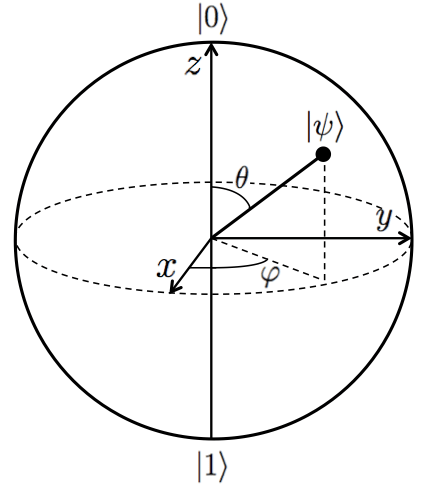
\includegraphics[scale=0.35]{img/EsferadeBloch.png}
    \caption{La esfera de Bloch representa todos los posibles estados cuánticos de un qubit.}
    \label{fig:esferaBloch}
\end{figure} \\
\noindent
Con esto en mente, podemos entender mejor cómo los qubits permiten realizar cálculos que son imposibles o ineficientes para las computadoras clásicas. Por ejemplo, mientras un bit clásico solo almacena un único valor en un momento dado, un qubit en superposición puede representar múltiples valores simultáneamente, aumentando exponencialmente la capacidad de procesamiento en ciertos tipos de problemas.\\[0.5em] 